\documentclass[a4,12Pt]{article}
\usepackage[utf8]{inputenc}
\usepackage{geometry}
 \geometry{
 a4paper,
 total={210mm,297mm},
 left=20mm,
 right=20mm,
 top=20mm,
 bottom=20mm,
 }
\usepackage{graphicx}
\begin{document}
\maketittle
\begin{flushright}
Artis Erglis\\
x141REB143\\
February 2015
\end{flushright}
\thispagestyle{empty}
\begin{center}
\large LD23H
\end{center}

\begin{flushleft}
Darba izpildes sakuma datums - 13.februaris\\
Darba pabeigšanas datums - 28.februaris
\end{flushleft}
\begin{center}
\section*{Atteli}
\end{center}
\begin{figure}[h]

\includegraphics[scale = 0.7]{231} 
\leftcaption{231.png - Sis ir izmēģinājuma atteels, punktu skaits 3x3}\\
\\

\includegraphics[scale= 0.5]{232} 
\leftcaption{232.png - Sis ir mans pirmais varda burts -A, punktu skaits 16x16}\\
\\

\includegraphics[scale= 0.5]{233} 
\leftcaption{233.png - Sie ir manai iniciaali: A un E, punktu skaits 32x32}\\
\\
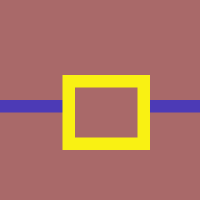
\includegraphics[scale= 0.7]{234} 
\leftcaption{234.png - Sis ir rezistora shematiskais apzimejums horizontali, punktu skaits 16x16}\\
\end{figure}
\clearpage
\begin{figure}[h]
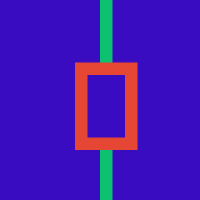
\includegraphics[scale= 0.7]{235} 
\leftcaption{235.png - Sis ir rezistora shematikais apzimejums vertikali, punktu skaits 16x16}\\
\\

\includegraphics[scale= 0.7]{236} 
\leftcaption{236.png - Sis ir spoles shematiskais apzimejums, punktu skaits 9x9}\\
\\

\includegraphics[scale= 0.7]{237} 
\leftcaption{237.png - Sis ir kondensatora shematiskais apzimejums, punktu skaits 9x9}\\
\\

\includegraphics[scale= 0.7]{238} 
\leftcaption{238.png - Sis ir sprieguma avota shematiskais apzimejums, punktu skaits 9x9}\\
\\

\includegraphics[scale= 0.7]{239} 
\leftcaption{239.png - Sis ir stravas avota shematiskais apzimejums, punktu skaits 9x9}
\pagebreak
\end{figure}
\clearpage
\begin{center}
\section*{Secinajumi}
\end{center}
\begin{flushleft}
Sajaa nedela es iemaacijos stradaat ar PythonMagick. Darbs bija interesants un reizee arii sarezgits.
\end{flushleft}
\end{document}
